\subsection{Revolute joint}\label{sec:CtrlExampleRevoluteJoint}
\begin{figure}[h!]
 \centering
 \input{graphics/RevoluteJoint.pdf_tex}
 \caption{Revolute joint: rigid body constrained to rotate about an axis}
 \label{fig:RevoluteJoint}
\end{figure}

\paragraph{Model.}
Another elemental case is the revolute joint, i.e.\ a rigid body constrained to rotate about an axis as illustrated on the left side of \autoref{fig:RevoluteJoint}.
With the joint angle $\jointAngle$ the rigid body configuration may be written as
\begin{align}
 \bodyHomoCoord{0}{1} = \begin{bmatrix} \cos\jointAngle & -\sin\jointAngle & 0 & 0 \\ \sin\jointAngle & \cos\jointAngle & 0 & 0 \\ 0 & 0 & 1 & 0 \\ 0 & 0 & 0 & 1\end{bmatrix}.
\end{align}
With the velocity coordinate $\sysVel = \jointAngled$ the equation of motion is
\begin{align}\label{eq:RevoluteJointModel}
 \Jzz \jointAngledd = \tau.
\end{align}

\paragraph{Potential energy.}
Due to the geometry of the model, only the control parameters $\Jczz, \sigczz, \kapczz \in \RealNum > 0$ contribute to the closed loop kinetics.
With the angle error $\jointAngleE = \jointAngle - \jointAngleR$ the potential may be written as
\begin{align}
 \potentialEnergyC = \kapczz (1 - \cos\jointAngleE).
\end{align}
It has the obvious transport map $\sysTransportMap = 1$.
The potential could be realized by attaching a single linear spring with stiffness $\sfrac{\kapczz}{\hcz^2}$ between desired configuration and actual configuration at a distance $\hcz$ as illustrated on the right side of \autoref{fig:RevoluteJoint}.
This also gives a vivid interpretation of the maximum on the potential at $\jointAngleE = \pm\pi$.

\paragraph{Approach 1.}
The particle based approach leads to the following closed loop kinetics
\begin{align}
 \label{eq:RevoluteJointClosedLoopApproachParticles}
%  \dissFktC = \tfrac{1}{2} \sigcz (\jointAngled^2 - 2\jointAngled \jointAngleRd \cos\jointAngleE + \jointAngleRd^2 ),
% \qquad
%  \kineticEnergyC = \tfrac{1}{2} \Jcz (\jointAngled^2 - 2\jointAngled \jointAngleRd \cos\jointAngleE + \jointAngleRd^2 )
% \\[1ex]
 \Jczz (\jointAngledd - \jointAngleRdd \cos\jointAngleE - \jointAngleRd^2 \sin\jointAngleE ) + \sigczz (\jointAngled - \jointAngleRd \cos\jointAngleE) + \kapczz \sin \jointAngleE = 0.
\end{align}
The total energy $\totalEnergyC$ and its time derivative are
\begin{subequations}
\begin{align}
 \totalEnergyC &= \tfrac{1}{2} \Jcz (\jointAngled^2 - 2\jointAngled \jointAngleRd \cos\jointAngleE + \jointAngleRd^2 ) + \kapcz (1 - \cos\jointAngleE),
\\
 \tdiff{t} \totalEnergyC 
%  &= \Jcz (\jointAngled \jointAngledd - \jointAngledd \jointAngleRd \cos\jointAngleE - \jointAngled \jointAngleRdd \cos\jointAngleE + \jointAngled \jointAngleRd \sin\jointAngleE (\jointAngled - \jointAngleRd) + \jointAngleRd \jointAngleRdd ) + \kapcz \sin \jointAngleE (\jointAngled - \jointAngleRd)
% \\
%  &= \big( \Jcz (\jointAngleRdd \cos\jointAngleE + \jointAngleRd^2 \sin\jointAngleE ) - \sigcz (\jointAngled - \jointAngleRd \cos\jointAngleE) - \kapcz \sin \jointAngleE \big) (\jointAngled - \jointAngleRd \cos\jointAngleE) 
% \\
%  &\qquad - \Jcz (\jointAngled \jointAngleRdd \cos\jointAngleE - \jointAngled \jointAngleRd \sin\jointAngleE (\jointAngled - \jointAngleRd) - \jointAngleRd \jointAngleRdd ) + \kapcz \sin \jointAngleE (\jointAngled - \jointAngleRd)
% \\
%  &= -\sigcz (\jointAngled - \jointAngleRd \cos\jointAngleE)^2 + \kapcz \jointAngleRd \sin \jointAngleE (\cos\jointAngleE - 1)
% \\ 
%  &\qquad \Jcz \big( \jointAngleRdd \jointAngled \cos\jointAngleE + \jointAngled \jointAngleRd^2 \sin\jointAngleE - \jointAngleRd \jointAngleRdd \cos^2 \jointAngleE - \jointAngleRd^3 \cos\jointAngleE \sin\jointAngleE
% \\
%  &\qquad - \jointAngled \jointAngleRdd \cos\jointAngleE + \jointAngled^2 \jointAngleRd \sin\jointAngleE - \jointAngled \jointAngleRd^2 \sin\jointAngleE + \jointAngleRd \jointAngleRdd \big)
% \\
 &= -\sigcz (\jointAngled - \jointAngleRd \cos\jointAngleE)^2 + \kapcz \jointAngleRd \sin \jointAngleE (\cos\jointAngleE - 1)
\nonumber\\
 &\qquad + \Jcz \jointAngleRd \big( \jointAngleRdd (1-\cos^2 \jointAngleE) + (\jointAngled^2  - \jointAngleRd^2 \cos\jointAngleE) \sin\jointAngleE \big)
\end{align} 
\end{subequations}
Without further assumptions on the reference trajectory $t \mapsto \jointAngleR(t)$ the total energy is \textit{not} a Lyapunov function for the closed loop.
The linear approximation $\jointAngle \approx \jointAngleR$ of \eqref{eq:RevoluteJointClosedLoopApproachParticles} has the characteristic polynomial
\begin{align}
 \lambda^2 + \tfrac{\sigcz}{\Jcz} \lambda + \big( \tfrac{\kapcz}{\Jcz} - \jointAngleRd^2 \big).
\end{align}
So even for the special case of constant reference velocity $\jointAngleRdd(t) = 0$, we need $\tfrac{\kapcz}{\Jcz} > \jointAngleRd^2$ to ensure local stability.

\paragraph{Approach 2 \& 3.}
For this example the body-based and energy-based approaches lead to identical energies and closed loop kinetics:
\begin{align}
 \dissFktC = \tfrac{1}{2} \sigczz \jointAngleEd^2,
\qquad
 \kineticEnergyC = \tfrac{1}{2} \Jczz \jointAngleEd^2,
\qquad
 \Jczz \jointAngleEdd + \sigczz \jointAngleEd + \kapczz \sin \jointAngleE = 0.
\label{eq:RevoluteJointClosedLoopApproachEnergy}
\end{align}
The total energy $\totalEnergyC = \kineticEnergyC + \potentialEnergyC$, $\totalEnergyCd = -2\dissFktC$ con be used to conclude that the system converges for \textit{almost} all initial conditions $(\jointAngleE(0), \jointAngleEd(0))$.
The remaining initial condition $\jointAngleE(0) = \pm\pi$ and $\jointAngleEd(0)=0$ is instable, see \autoref{fig:PhasePlotSO2}.
As a physical interpretation: the controlled dynamics coincide with the dynamics of a damped physical pendulum.

\paragraph{Linear control.}
Since the model \eqref{eq:RevoluteJointModel} is a linear differential equation, the following linear closed loop equation might also be reasonable
\begin{align}\label{eq:RevoluteJointCtrlLin}
 \Jczz \jointAngleEdd + \sigczz \jointAngleEd + \kapczz \jointAngleE = 0.
\end{align}
The difference between the closed loop \eqref{eq:RevoluteJointClosedLoopApproachEnergy} and \eqref{eq:RevoluteJointCtrlLin} may be visualized by the corresponding phase plots, see \autoref{fig:PhasePlotSO2}:
The linear control law leads to non-smooth phase curves at $\jointAngle = \pm\pi$, which is the consequence of the linear design for a system whose configuration space is actually $\Sphere^1 \ncong \RealNum$.
See \cite[sec.\ 1.2]{Konz:AT} for a deeper discussion.

\begin{figure}[ht]
 \centering
 \input{graphics/PhasePlotSO2.pdf_tex}
 \caption{Phase plot for \eqref{eq:RevoluteJointClosedLoopApproachEnergy}, left, and for \eqref{eq:RevoluteJointCtrlLin}, right}
 \label{fig:PhasePlotSO2}
\end{figure}

\paragraph{Simulation results.}
\autoref{fig:RevoluteJointSimRes} shows simulation results comparing the three different approaches \eqref{eq:RevoluteJointClosedLoopApproachParticles}, \eqref{eq:RevoluteJointClosedLoopApproachEnergy} and \eqref{eq:RevoluteJointCtrlLin} tracking a reference $\jointAngleR(t) = \tfrac{\pi}{2}\sin(\tfrac{2\pi}{2.5}t)$.
Evidently, all approaches fulfill the control objective, i.e. the joint angle $\jointAngle$ converges to its reference $\jointAngleR$.
\begin{figure}[ht]
 \centering
 \appendtographicspath{{graphics/RevoluteJoint/}}
 \begingroup%
\setlength{\unitlength}{1cm}%
\begin{picture}(15.900000,10.000000)%
\put(0,0){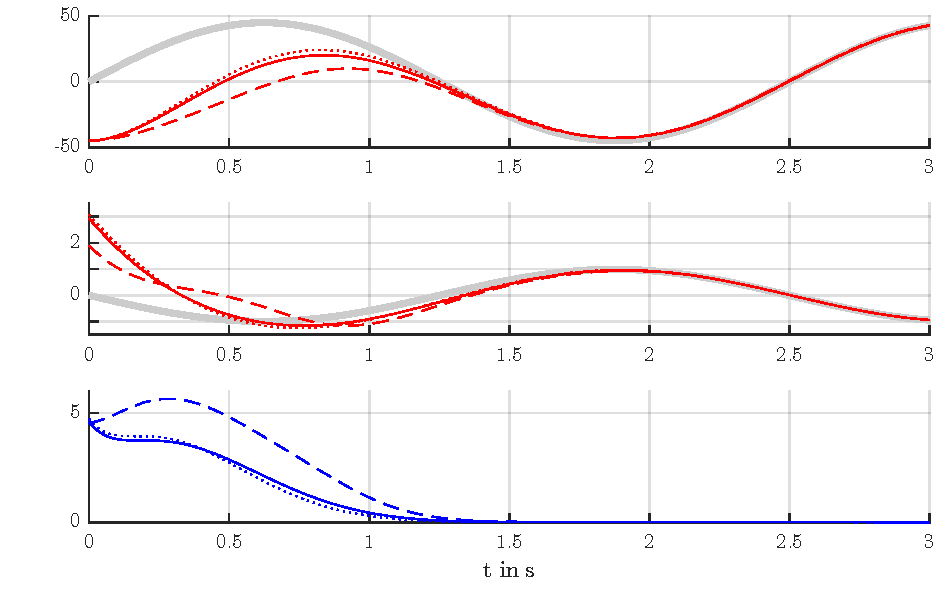
\includegraphics{RevoluteJointSimRes.pdf}}%
\put(0.942384, 2.252072){\rotatebox{90}{\makebox(0,0)[t]{\smash{$\totalEnergyC$ in $\unit{J}$}}}}%
\put(0.942384, 5.425047){\rotatebox{90}{\makebox(0,0)[t]{\smash{$\tau$ in $\unit{Nm}$}}}}%
\put(0.648402, 8.598021){\rotatebox{90}{\makebox(0,0)[t]{\smash{$\jointAngle$ in $\unit{DEG}$}}}}%
\end{picture}%
\endgroup%
 \caption{Simulation result for the revolute joint: gray line: reference, dashed line: particle-based approach, solid line: energy-based approach, dotted line: linear approach}
 \label{fig:RevoluteJointSimRes}
\end{figure}
